% !TEX root =  ../report.tex

\section{Implementation}
\label{s:impl}
The source code for the OP2 Framework is hosted open source as a GitHub\cite{OP2rep} repository. Instructions for obtaining the implementation described in the following section, and for getting started with OP2, are provided be found in Appendix \ref{app:getStart}.
\subsection{Git Repository}
The feature branch for this project is named \verb|feature/jit|, and was branched from \verb|feature/lazy-execution| on 13th November 2019. The last commit on the \verb|lazy-execution| was in April 2018, and therefore lagged behind the \verb|master| branch somewhat. It was rebased onto \verb|master| before any other changes were made.
\par
In git terminology, a rebase involves making copies of a branch's commits, and "re-playing" the changes made in them to the top of another branch \cite{scm-rebase}. In this case, making copies of all commits made to \verb|feature/lazy-execution| and applying them to the latest commit of \verb|master|. The result once any merge conflicts are resolved will be a codebase with all the features of both branches available.
\begin{figure}[h!]
  \caption{Rebase vs. Merge. Diagram reproduced from \cite{scm-rebase}}
  \label{fig:git_merge}
  \makebox[\textwidth][c]{
  \resizebox{1.1\textwidth}{!}{
    \begin{tikzpicture}[node distance=3.5cm, auto]

      %
      % Initial
      %

      \tikzstyle{label} = [rblock, text width=7em, minimum height=2em, fill=green!30]

      \node [wfile] (C0) {C0};
      \node [wfile, right of=C0] (C1) {C1};
      \node [wfile, right of=C1] (C2) {C2};
      \node [jfile, above=1cm of C2] (C3) {C3};
      \node [label, above=1cm of C3] (fhead) {feature/HEAD};
      \node [label,  below=1cm of C2] (mhead) {master/HEAD};

      \node [above=2em of C0] (initial) {\LARGE Initial State};

      \path [line] (C1) -- (C0);
      \path [line] (C2) -- (C1);
      \path [line] (C3.south west) -- (C1.north east);
      \path [thinline] (fhead) -- (C3);
      \path [thinline] (mhead) -- (C2);

      %
      % Rebase
      %

      \node [wfile, below=6cm of C0] (fC0) {C0};
      \node [wfile, right of=fC0] (fC1) {C1};
      \node [wfile, right of=fC1] (fC2) {C2};
      \node [jfile, above=1cm of fC2, opacity=0.2] (fC3) {C3};
      \node [label, below=1cm of fC2] (fmhead) {master/HEAD};

      \node [above=2em of fC0] (rebase) {\LARGE Rebased Commits};

      \node [jfile, right of=fC2] (fC3prime) {C3'};
      \node [label, above=1cm of fC3prime] (ffhead) {feature/HEAD};

      \path [line] (fC1) -- (fC0);
      \path [line] (fC2) -- (fC1);
      \path [line, opacity=0.2] (fC3.south west) -- (fC1.north east);
      \path [thinline] (ffhead) -- (fC3prime);
      \path [line] (fC3prime) -- (fC2);
      \path [thinline] (fmhead) -- (fC2);

      %
      % Merge
      %

      \node [wfile, right=3cm of fC3prime] (mC0) {C0};
      \node [wfile, right of=mC0] (mC1) {C1};
      \node [wfile, right of=mC1] (mC2) {C2};
      \node [jfile, above=1cm of mC2] (mC3) {C3};
      \node [label, above=1cm of mC3] (mfhead) {feature/HEAD};

      \node [wfile, right of=mC2] (mC4) {C4};
      \node [label, below=1cm of mC4] (mmhead) {master/HEAD};

      \node [above=2em of mC0] (merge) {\LARGE Merged Commits};

      \path [line] (mC1) -- (mC0);
      \path [line] (mC2) -- (mC1);
      \path [line] (mC3.south west) -- (mC1.north east);
      \path [line] (mC4) -- (mC2);
      \path [line] (mC4.north west) -- (mC3.south east);
      \path [thinline] (mfhead) -- (mC3);
      \path [thinline] (mmhead) -- (mC4);

    \end{tikzpicture}
    }}
\end{figure}
\par
Rebasing is preferable to simply merging for integrating another branch's changes as the result is a linear branch history, rather than creating a diamond. Also, in the case of merge conflicts - where a change has been made in both branches and one needs to be selected - a rebase command will stop at the first conflicting commit and allow the conflict to be resolved \cite{rebase-doc}. Synchronising using merge would result in receiving all conflicts in one go, which can make it harder to resolve.
\par
The downside of rebasing is it can be harder to recover from an erroneous rebase, than an erroneous merge. This is due to the fact that merges are not destructive, since they do not re-write history in the same way as a rebase. This will not be an issue here however.
\par
The \verb|feature/lazy-execution| branch was created for developing a system to execute parallel loops when values are required, rather than when they are called. This functionality will be achieved using an internal library function:
\codeline{void op_enqueue_kernel(op_kernel_descriptor *desc)}{op2/c/src/core/op\_lazy.cpp [71-89]}
Currently this function executes the queued loop as soon as it is invoked, but there is ongoing work into determining when the result of the loop will be needed, and potentially compressing multiple queued actions into fewer at this time. Lazy execution will not be the focus of this project, however the process for invoking parallel loops will be utilised throughout the work done to enable Just-In-Time Compilation for CUDA, so that future efforts towards lazy execution can continue on top of the JIT compilation implementation.

\subsection{Code Generation}
\label{ss:codegen}
As described in the Specification before, the majority of the implementation work can be found in a Python code generation script which can be found inthe folder: \verb|translator/c/python/jit/op2_gen_cuda_jit.py| of the OP2 repository.
\noindent The code generator for CUDA with JIT compilation is called from another Python script named \verb|op2.py|, which can be found in the parent directory: \verb|translator/c/python/|. This script handles the generation of the Modified Application File, which does not need to change to meet the requirements of this project. The following section will summerise the functionality of \verb|op2.py|, to assist in understanding the context for the CUDA code generation script.

\subsubsection{op2.py}
\verb|op2.py| is a pre-existing script in the OP2 Framework, which processes application files to gather information to pass to each of the platform specific code generator scripts. It uses Python Regular Expressions to identify OP2 API calls, and ensures certain conditions are met - for example that \verb|op_init| and \verb|op_exit| are called at least once.
\par
It also gathers information about each parallel loop, including the number and type of the parameters, and the details of the indirect data set if the loop is indirect. This stage also includes some error checking, by ensuring types and dimensions are coherent throughout the application.
\par
Once the Application has been analysed, the application file is modified to produce \verb|[-application]_op.cpp|, which is mostly the same as the original application file, but with the addition of \verb|extern| declartions for the function each parallel loop will call: \verb|op_par_loop_[name]|. An implementation for this function will be generated for each hardware platform, including for CUDA with Just in Time compilation - which is the code generator for this project.
\par
Each code generator receives the list of kernel details for each parallel loop as a parameter when it is invoked.

\subsubsection{jit/op2\_gen\_cuda\_jit.py}
The entry point function for the CUDA JIT code generation is:
\pyline{op2_gen_cuda_jit(master, date, consts, kernels)}{translator/c/python/jit/op2\_gen\_cuda\_jit.py [102]}
\noindent The arguments passed to it from \verb|op2.py| are:
\begin{center}
\begin{tabular}{>{\bfseries}l l}
master: & The name of the Application file \\[\medskipamount]
date: & The exact date and time of code generation \\[\medskipamount]
consts: & list of constants, with their type, dimension and name \\[\medskipamount]
kernels: & \parbox[t]{.8\textwidth}{list of kernel descriptors, where each element is a map containing many fields describing the kernel.} \\[\medskipamount]
\end{tabular}
\end{center}
\vspace{1em}
\noindent Where the \verb|kernels| argument serves as the primary input, that the output will be most affected by. The output will be two C source code files, referred to as \textbf{kernel files}, for each parallel loop. They will have the following naming scheme:
\begin{itemize}
\vspace{-.5em}
\item{AOT: \verb|cuda/[name]_kernel.cu|}
\vspace{-.5em}
\item{JIT: \verb|cuda/[name]_kernel_rec.cu|}
\end{itemize}
A single \textbf{central kernels file} is also generated, which is shared between all parallel loops:
\begin{itemize}
\vspace{-.5em}
\item{\verb|cuda/[application]_kernels.cu|}
\end{itemize}
It will contain function definitions required by all loops, or by the master application file; as well as include statements for each of the parallel loops' AOT kernels so they are collated into a single file by the compiler.
\par
The first action of the code generator is to perform a check across all kernels to see if any use the Struct of Arrays data layout \cite[p13]{manual}, or if all are using the default Array of Structs. Then, a folder \verb|cuda/| is created if it doesn't already exist, and the script will iterate over each kernel, generating both the Ahead-Of-Time (AOT) kernel file, and the Just-In-Time (JIT) kernel file simultaneously. In the System Digram from Section \ref{s:spec} (Figure \ref{fig:jit_sys}) these files were referred to as "Kernels" and "Optimised Kernels" respectively.

\subsubsection{Kernel Files}
\label{ss:krnl_files}
As mentioned above, the code generator outputs two C source code files for each parallel loop. The following section steps through these kernel files, explaining the purpose of each function that will be generated, and therefore covering a large part of the implementation.
\par To avoid confusion, Python code that a segment of the implementation will be marked with just a file and line reference, and C code that is an output will be marked \textit{generated by ...} and then a file and line reference.
\par
Figures \ref{fig:jit_include}-\ref{fig:loop_func} show the progression of the two kernel files for an typical parallel loop, and there is a summary on page \pageref{impl_summary} if the detail is superfluous for your needs.
\par
It may aid in understanding to follow this section with either the translations script, or a set of generated kernel files to hand, since it would not be practical to include full code listings on each page. The inclusion of Figures \ref{fig:jit_include}-\ref{fig:loop_func} is only for purposes of highlighting the relevant sections of each file, and the generated code in the figures is not intended to be a legible size.

% May need to move
\clearpage
%
\begin{wrapfigure}[21]{r}{.33\textwidth}
  \centering
  \caption{JIT includes}
  \label{fig:jit_include}
  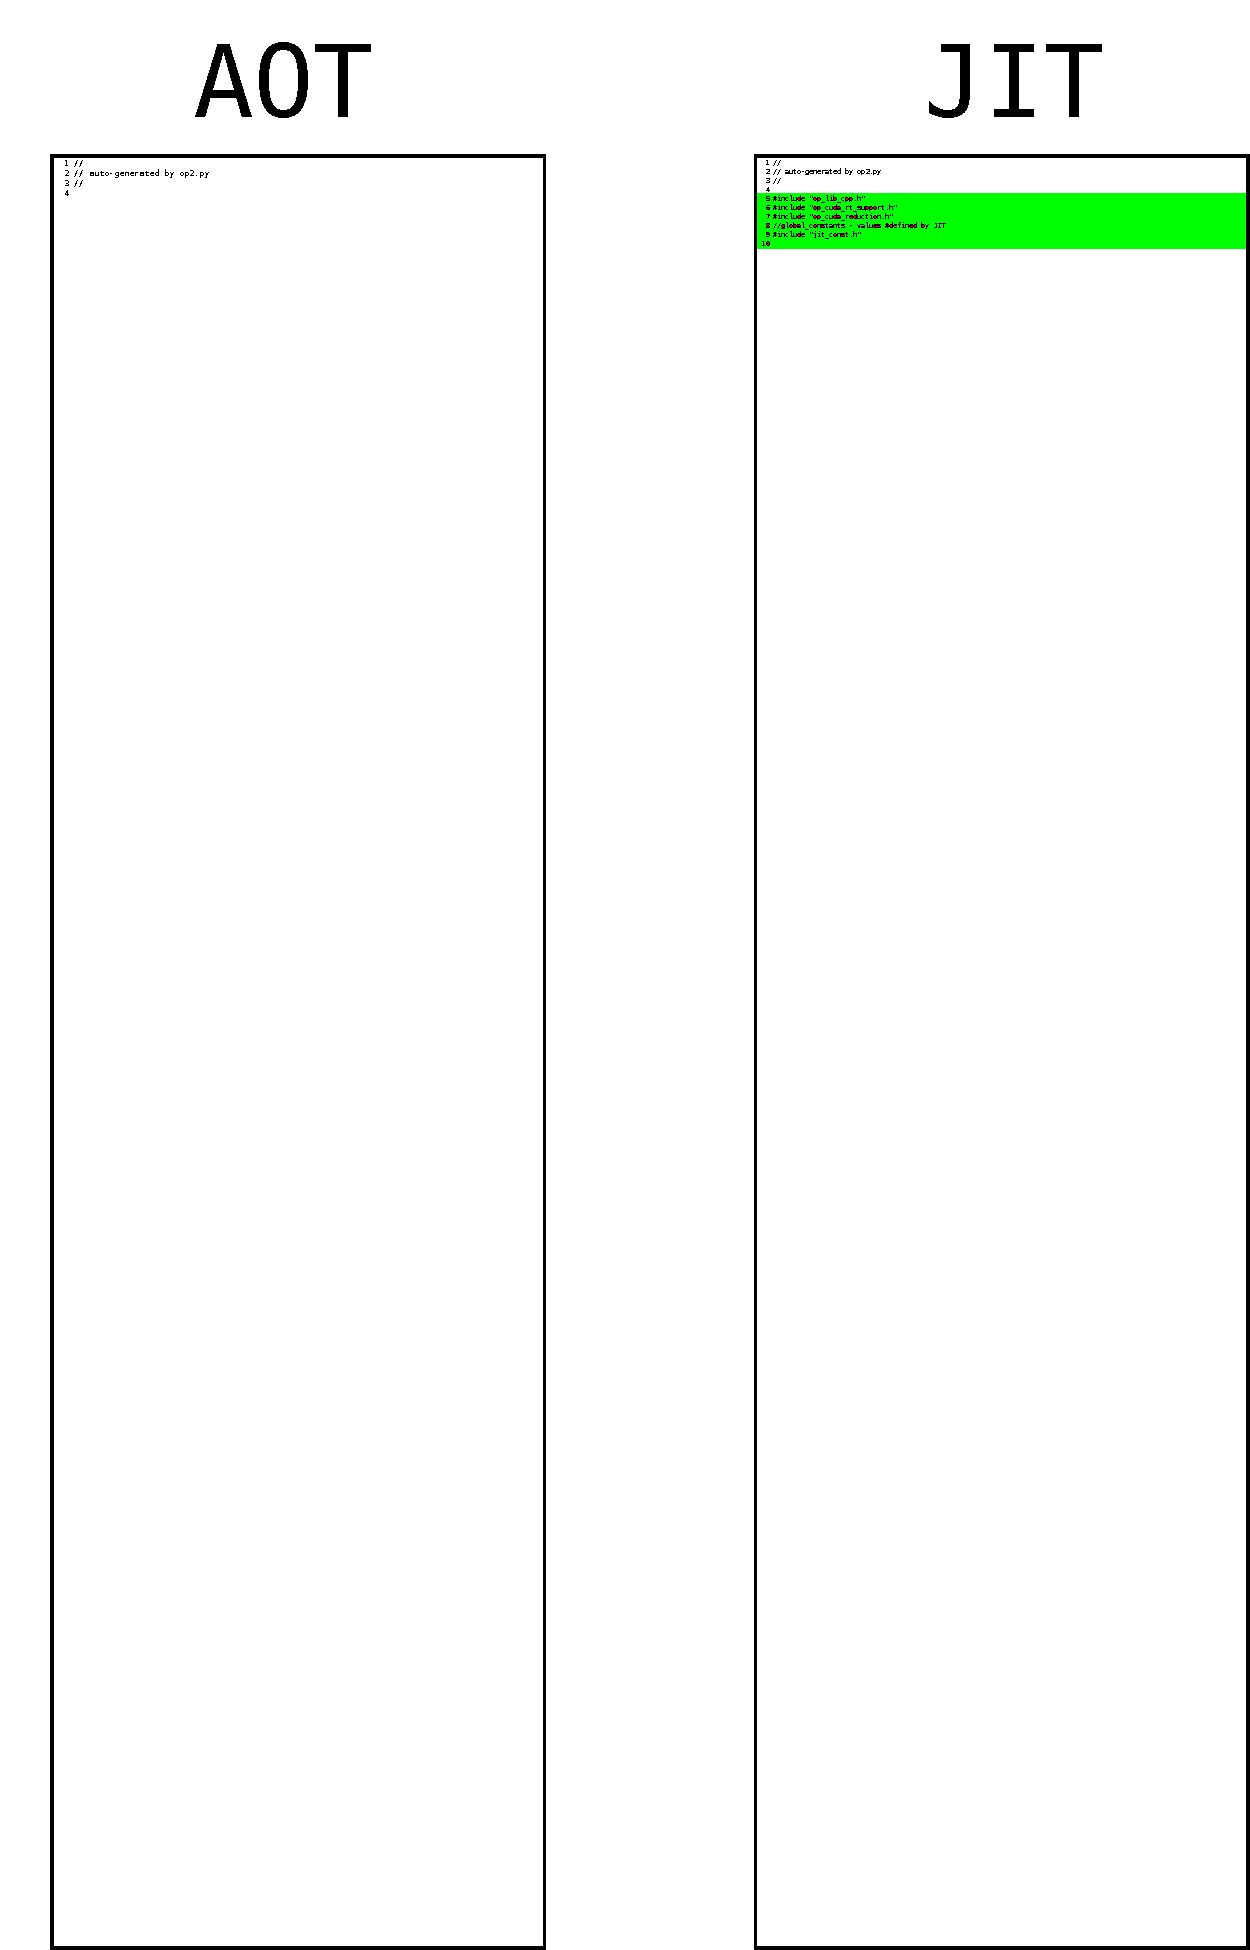
\includegraphics[width=.3\textwidth]{jit_include}
\end{wrapfigure}
\minititle{JIT includes}
The first piece of C code generated by the Python script is simply the include directives required for the JIT compiled kernel. These are needed for JIT compiled kernels since they will be processed individually by the compiler, so each requires a reference to the OP2 library files. They are not needed by the AOT kernel, as they will be included in the central kernels file, which in turn includes each of the AOT kernel files to produce a single file with all of the AOT kernels and these same \verb|#include| statements:
\begin{lstlisting}[backgroundcolor = \color{green!20}, language=C]
 #include `op_lib_cpp.h'
 #include `op_cuda_rt_support.h'
 #include `op_cuda_reduction.h'
 ...
\end{lstlisting}
\codelabel{generated by TODO}
The \verb|jit_const.h| file is also included, which will be generated at run-time (before the compiler is invoked) to contain a \verb|#define| for all input constants, to be handled by the pre-processor.
\begin{lstlisting}[backgroundcolor = \color{green!20}, language=C]
 ...
 //global_constants
 #include `jit_const.h'
\end{lstlisting}
\codelabel{generated by TODO}

\minititle{User Function}
The User Function is the kernel operation specified by the user to be carried out on each iteration of the loop, so this function will run on the device (GPU) on many threads simultanously, performing an action at least once for each set item.

\begin{wrapfigure}[12]{r}{.33\textwidth}
  \centering
  \caption{User Function}
  \label{fig:usr_func}
  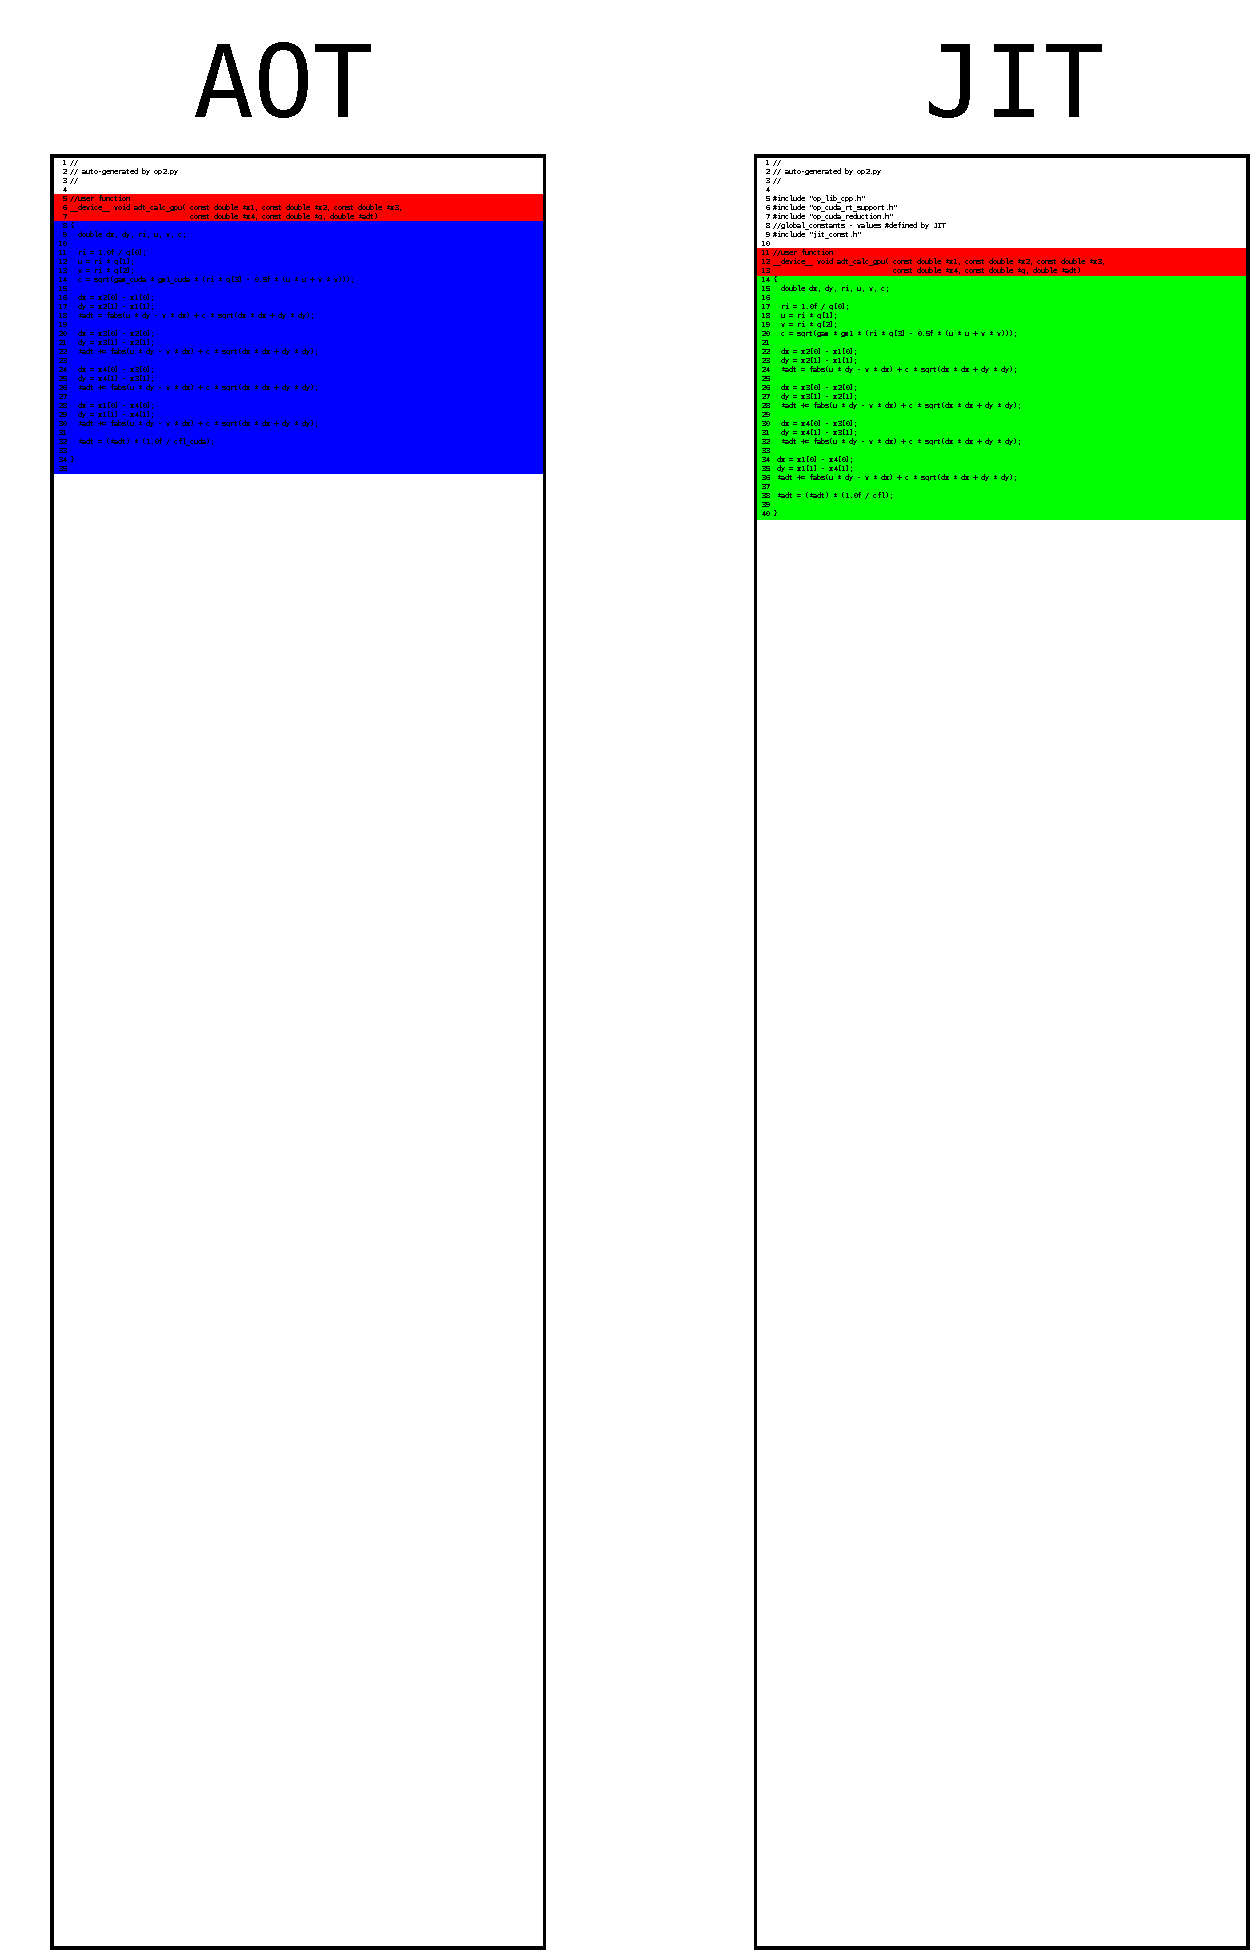
\includegraphics[width=.3\textwidth]{user_function}
\end{wrapfigure}
The User Function is given the \verb|__device__| function  descriptor, so that it will be compiled for execution on a GPU device, and can only be called from other device code - which will be the next function generated. The whole signature for the function will be:
\codeline{__device__ void [name]_gpu ( [args] )}{}
\noindent The function body will be pulled from either the application file or a header file, and is checked to ensure it has the correct number of parameters. Any include statements are replaced by the contents of the file, exactly as the pre-processor would.
\par
\tinytitle{Data Layout} If the Struct of Arrays data layout is not requested, the function body will remain largly the same as defined by the application programmer. If it is enabled however there are modifications that need to be made to support this. The code to do this is pulled from the AOT CUDA code generation script: \\\verb|translator/c/python/aot/op2_gen_cuda_simple.py|.
\par
Since the modifications involve constant values for the stride of different data structures, an attempt to streamline this process using the same constant definition optimisation was made during this project. It was unsuccessful, with a longer discussion on why later in the report.
\par
\tinytitle{Optimisations} The constant definition optimisation only needs to be applied to the user function, as it is the only one containing code written by the application developer. Wherever an input constant is referenced it needs to be modified in both the AOT and JIT kernel, but in different ways.

\tinytitle{AOT}
In the Ahead-Of-Time kernel, which will only be executed if JIT compilation is disabled, the constant will need to read from the device's memory - having been copied there when it is defined constant. The copied version will have the identifier \verb|[id]_cuda| to prevent a name collision, so all constants in the AOT kernel must be replaced with this pattern, using the following lines from the translator script:\\
\begin{lstlisting}[backgroundcolor = \color{lightgray!20}, language=Python]
for nc in range(0,len(consts)):
  varname = consts[nc]['name']
  aot_user_function = re.sub('\\b' + varname + '\\b',
                              varname + '_cuda',
                              aot_user_function)
\end{lstlisting}
\codelabel{translator/c/python/jit/op2\_gen\_cuda\_jit.py [905-907]}

\tinytitle{JIT}
The JIT kernel is a little different: contants with a dimension of 1 (i.e. they contain only 1 value) can be left the unchanged, as the value will be defined under that same identifier. There is no chance of a name collision here since the idenifier will never be allocated memory, only replaced by a literal value.
\par
Multi-Value proved more of a challenge - since values cannot be declared both \verb|__constant__| and defined as external using \verb|extern| \cite[p126]{guide}, which is how they are handled for the sequential JIT implementation.
\par
The eventual solution to this challenge was in two parts. For each index \verb|N| of the constant array, a 1 dimensional constant would be defined with the name: \verb|op_const_[id]_[N]|. All references to the constant where the index is a literal number can be replaced with the new identifier:
\begin{lstlisting}[backgroundcolor = \color{lightgray!20}, language=Python]
for nc in range(0,len(consts)):
  varname = consts[nc]['name']
  if consts[nc]['dim'] != 1:
    jit_user_function = re.sub(`\\b' + varname + `\[([0-9]+)\]',
                               `op_const_' + varname + `_\g<1>',
                                jit_user_function)}
\end{lstlisting}
\codelabel{translator/c/python/jit/op2\_gen\_cuda\_jit.py [931-934]}

If the constant is accessed using any expression other than a integer literal, this system will run into an issue. As an example, see the result of processing the following statement, where \verb|c_array| is a defined constant with dimension greater than 1:
\begin{center}
\lstinline|int A = c_array[1 + 2]| \space{1cm}$\Rightarrow$\space{1cm} \lstinline |int A = op_const_c_array_1 + 2|
\end{center}

If this problem is not solved the most likely outcome is an undefined indentifier error at compile time. In the above example the code will actually compile, but clearly the whole meaning of the statement has changed from the developer's intention, as \verb|op_const_c_array_1| will be replaced by the first value in the array then the literal integer value of 2 will be added to it.
\par
To resolve this, a constant device array is declared in global scope above the top of the function, with the identifier \verb|op_const_[name]|. Each index of the array will be the constant defined for that position. The accesses then can still use the expression for an index, but are modified to instead access the new array, instead of the constant's identifier - so that the meaning of the statement is preserved.
\par This is only done when an expression index is found and the process becomes necessary, since allocating a new array can take time. If there are no expression accesses, the code will not be generated to handle them.
\begin{lstlisting}[frame=none,backgroundcolor=\color{white}]

__constant__ int op_const_c_array = { op_const_c_array_1, ...}
 ...
int A = op_const_c_array[1+2]
\end{lstlisting}
The above is a trivial example, and the actual code is unlikely to be an expression involving only literal values. If it were, then there would be benefit to implementing constant folding to evalute the expression where possible, but this was not done due to the unlikely nature of such code actually being executed.
\par

On the next page is the full Python code for the JIT compiled kernel constants.
\clearpage
\begin{lstlisting}[backgroundcolor = \color{lightgray!20}, language=Python]
for nc in range(0,len(consts)):
  varname = consts[nc]['name']
  if consts[nc]['dim'] != 1:
    # Replace all instances with literal int index
    jit_user_function = re.sub('\\b'+varname+'\[([0-9]+)\]',
                               'op_const_'+varname+'_\g<1>',
                                jit_user_function)

    # Replace and count all remaining array accesses
    jit_user_function, numFound = re.subn('\\b'+varname+'\[',
                                          'op_const_'+varname+'[',
                                           jit_user_function)

    # At least one expression index was found
    if (numFound > 0):
      if CPP:
        #Line start
        codeline = '__constant__ '           +\
                    consts[nc]['type'][1:-1] +\
                   ' op_const_'              +\
                    varname                  +\
                   '[' + consts[nc]['dim'] + '] = {'

        #Add each constant index to line
        for i in range(0,int(consts[nc]['dim'])):
          codeline += "op_const_"+varname+"_"+str(i)+", "

        # Remove last comma, add closing brace
        codeline = codeline[:-2] + "};"

        #Add array declaration above function
        jit_user_function =  codeline +\
                            '\n\n'    +\
                             jit_user_function
\end{lstlisting}
\codelabel{translator/c/python/jit/op2\_gen\_cuda\_jit.py [931-944 UPDATE]}
\clearpage
\begin{wrapfigure}[14]{r}{.33\textwidth}
  \centering
  \caption{Kernel Function}
  \label{fig:krnl_func}
  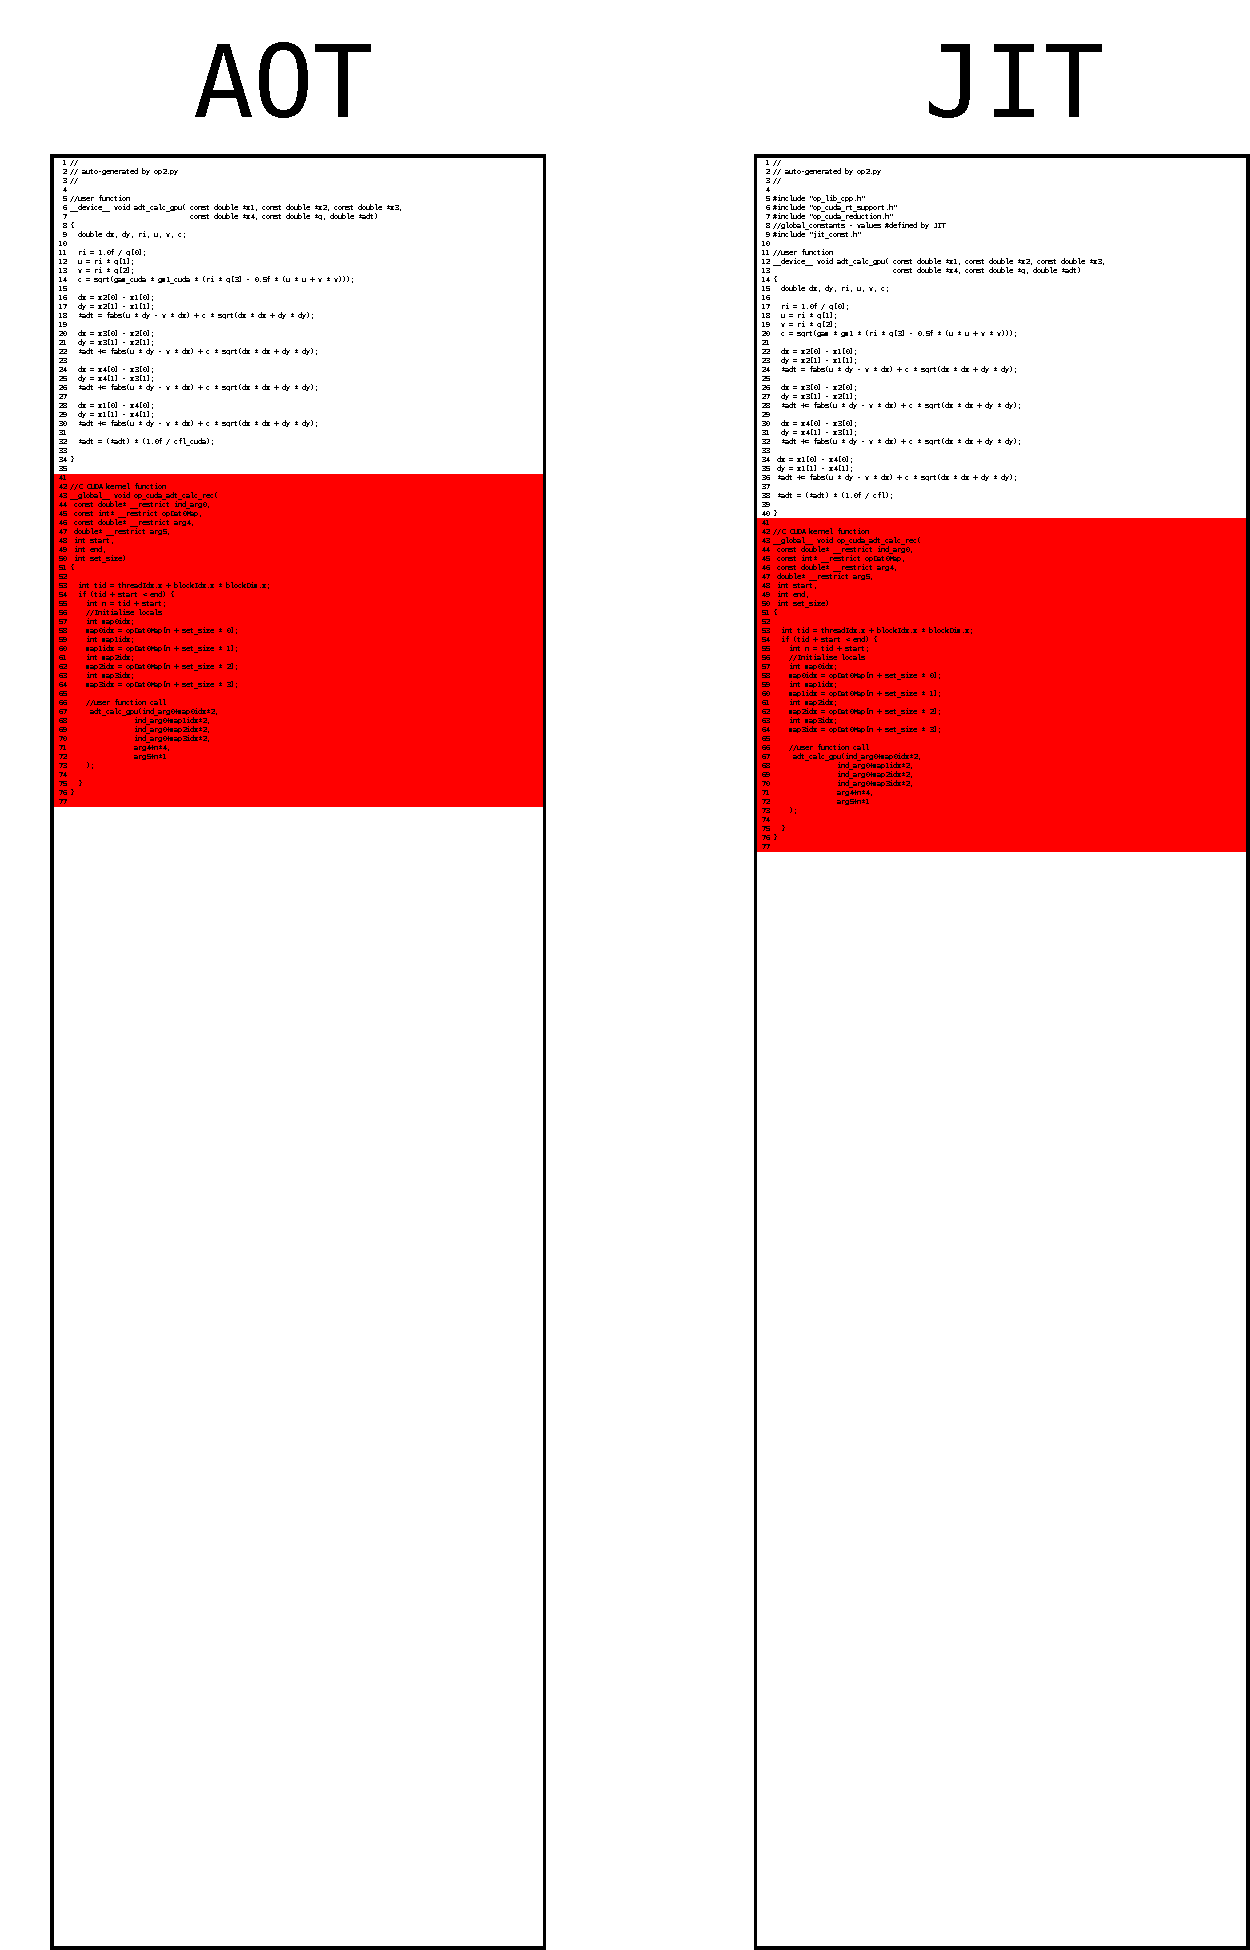
\includegraphics[width=.3\textwidth]{kernel_function}
\end{wrapfigure}
\minititle{Kernel Function}
From here onward, all code generated is based only on the kernel descriptor, and does not contain any code written by the application developer.
\par The kernel function is the same in both files, and is also executed on the GPU across all the parallel threads. It is declared \verb|__global__| so that is exectuted on the device, but can be called from host (CPU) code:
\codeline{__global__ void op_cuda_'+name+'( [args] )}{}
The purpose of this function is to use the CUDA built in variables \verb|threadIdx.x|, \verb|blockIdx.x|, and \verb|blockDim.x| to determine which section of the workload should be done by each thread. These variables allow a thread to identify iteself from others.

\tinytitle{Indirection} If the loop is indirect, and uses values from another map as indicies, these values need to be read from the inner map in this function, so that the User Function (generated above) can receive all the data it needs without needing to process it. It is possible that the indirect mapping could be optional, in which case the \verb|optflags| argument is checked using a bit comparison to determine if the optional argument was passed or not.
\par
Once this is done, a call is then made to the user function with the parameters it requries, followed by performing any reductions that need to be done. The supported reductions are: sum, maximum, and minimum\cite[p11]{manual}. Reductions are handled by the \verb|op_reduction| library function.

\begin{wrapfigure}[8]{r}{.33\textwidth}
  \centering
  \caption{Host Function}
  \label{fig:host_func}
  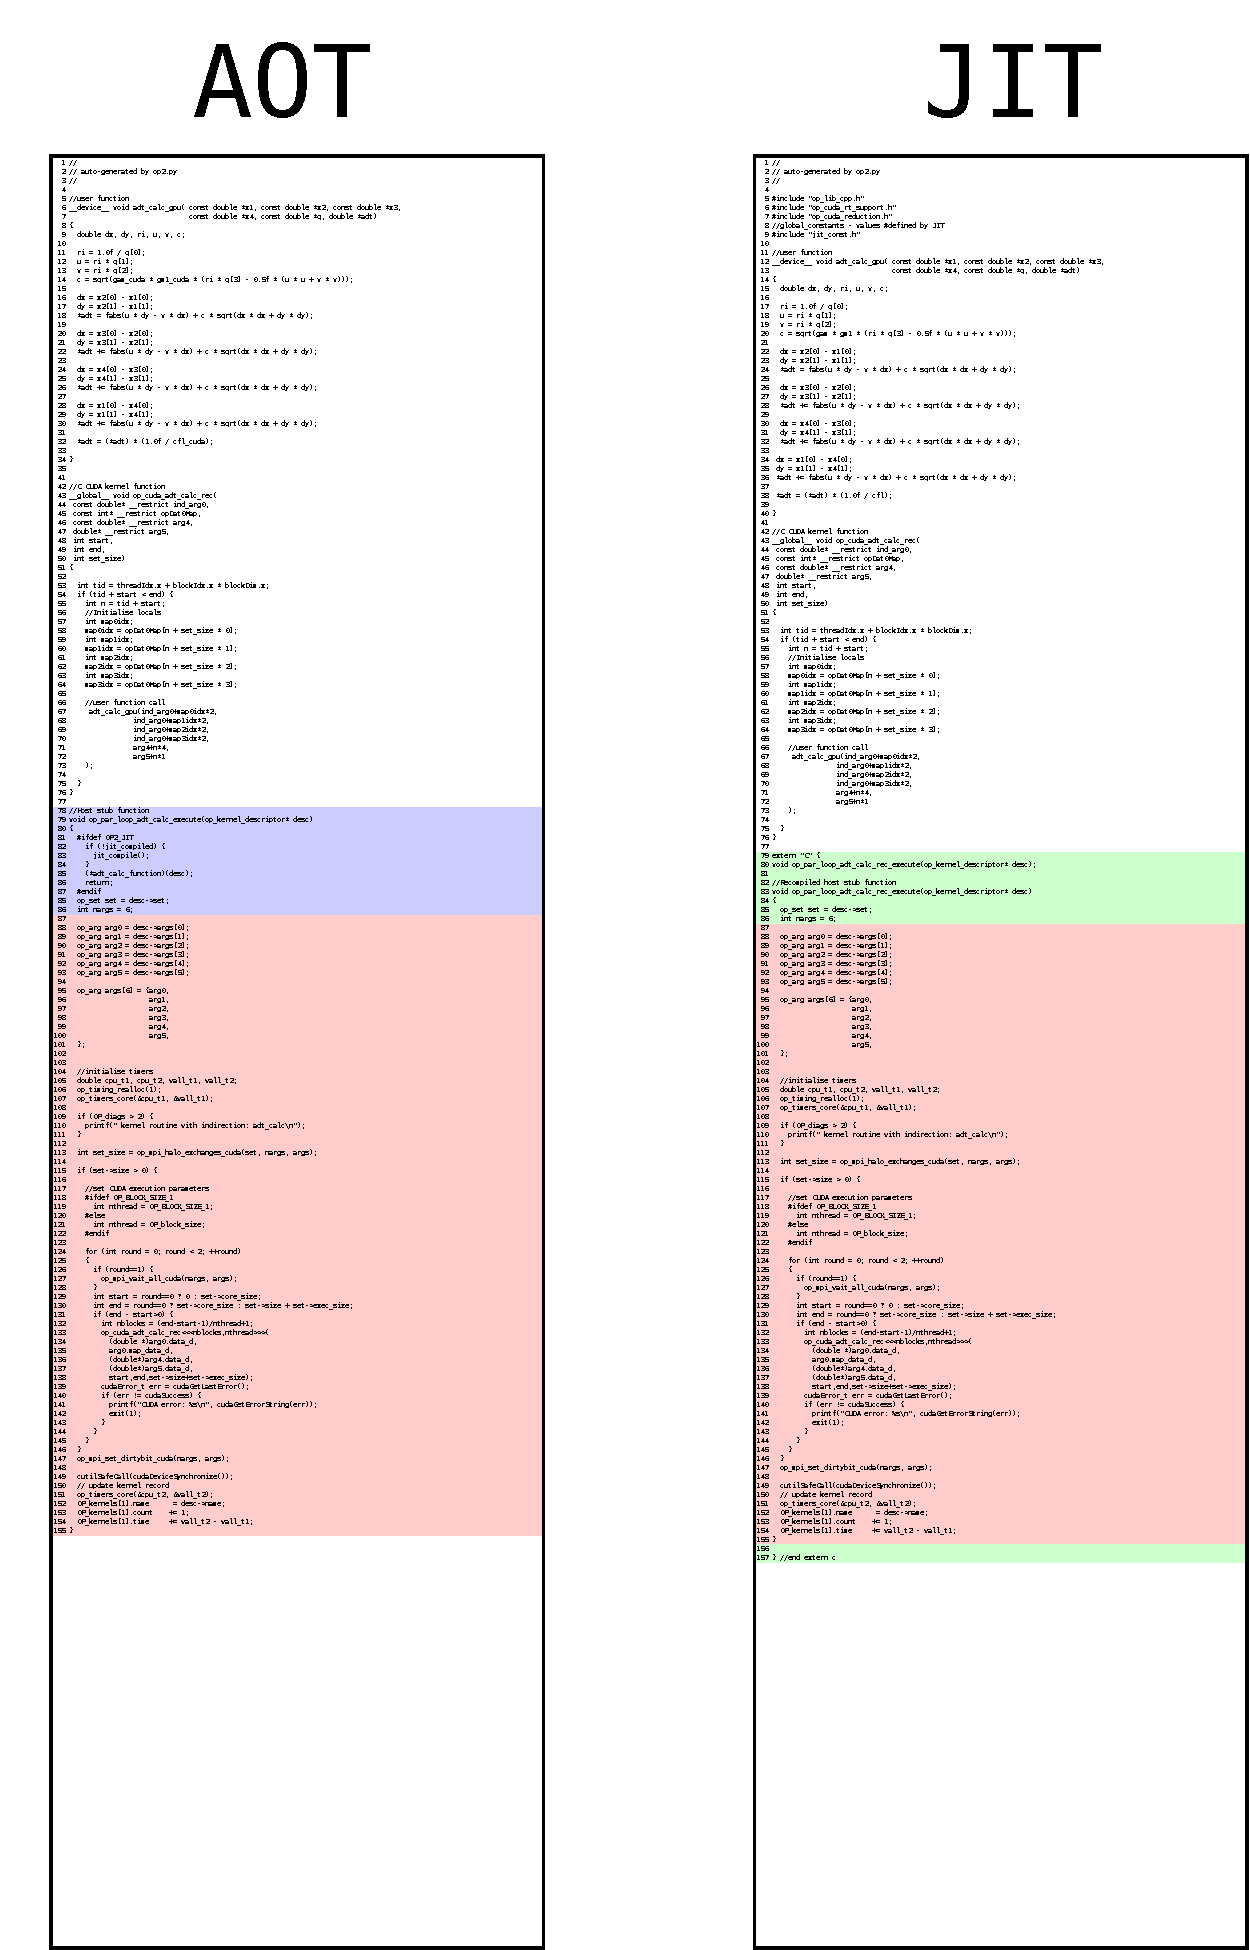
\includegraphics[width=.3\textwidth]{host_function}
\end{wrapfigure}
\minititle{Host Function}
The purpose of the host function is to bridge the gap between the host and the device. It is CPU code, so runs on the host, but contains the CUDA call to the kernel function which will run on the GPU. While the function body is the same for both AOT and JIT: setting up arguments, timers, and block and thread sizes for the CUDA call; the function head differs, as highlighted in Figure \ref{fig:host_func}.
\vspace{\parskip}

\tinytitle{AOT}
In the Ahead-Of-Time kernel file, the C code generated for the head of the host function is as follows:

\begin{lstlisting}[linewidth = \textwidth, framesep=0pt, language=C, linebackgroundcolor={\ifnum\value{lstnumber}<15 \ifnum\value{lstnumber}>10 \color{red!20} \else \color{blue!20} \fi \else \color{blue!20} \fi}]
 //Host stub function
 void op_par_loop_[name]_execute(op_kernel_descriptor* desc)
 {
   #ifdef OP2_JIT
     if (!jit_compiled) {
       jit_compile();
     }
     (*[name]_function)(desc);
     return;
   #endif

   op_set set = desc->set;
   int nargs = 6;
   ... //Identical Section
 }
\end{lstlisting}

\codelabel{Generated by translator/c/python/jit/op2\_gen\_cuda\_jit.py [537-558]}

The function name is \verb|op_par_loop_[name]_execute| because a pointer to this function will be queued by the lazy execution system mentioned previously in this Section, so this function actually executes the loop, whenever the lazy execution system should decide it needs to be executed. The decision of when to call the loop is outside the scope of this project, and currently a loop is simply called immediately after it is queued.
\par At the top of the function a decision is made as to whether JIT should be used, based on whether the pre-processor flag with identifier \verb|OP2_JIT| has been defined. This allows JIT to be enabled by passing the compiler \verb|-DOP2_JIT| as an argument, and otherwise by default it will be disabled. If JIT is enabled, then the compiler is invoked (if it hasn't been already), and the pointer to the newly compiler version of the function is executed instead.
\par
If JIT is not enabled, this code will be ignored by the compiler, so the process will continue into the AOT host function, which causes it to stay whithin the AOT kernel file and never execute any code from the JIT file.

\tinytitle{JIT}
Contrasting this with the code generated for the JIT kernel file:

\begin{lstlisting}[linewidth = \textwidth, framesep=0pt, linebackgroundcolor={\ifnum\value{lstnumber}<10 \ifnum\value{lstnumber}>6 \color{red!20} \else \color{green!20} \fi \else \color{green!20} \fi}]
 extern "C" {
 void op_par_loop_[name]_rec_execute(op_kernel_descriptor* desc);

 //Recompiled host stub function
 void op_par_loop_[name]_rec_execute(op_kernel_descriptor* desc)
 {
   op_set set = desc->set;
   int nargs = 6;
   ... //Identical Section
 }

 } //end extern c
\end{lstlisting}

\codelabel{Generated by translator/c/python/jit/op2\_gen\_cuda\_jit.py [522-531]}

Firstly, since this function needs to be linked to the exisiting code as part of a dynamically loaded library, it is placed inside an \verb|extern "C"| scope, to ensure C language function linkage, and prevent the compiler from "mangling" the name as it would for C++ code \cite{linkage}. Following that, the function, which is named\\
\verb|op_par_loop_[name]_rec_execute| ("rec" short for recompiled), will come to reside at the address pointed to by the \verb|[name]_function| function pointer previously referenced in the AOT kernel.
\par
It will be executed after the run-time compiler has been invoked, as the replacement JIT-compiled host function, and since it makes calls to the kernel and user functions in the same file as iteself, rather than those in the AOT file, the optimisations made to the user function in the JIT kernel are able to be used.

\tinytitle{SOA}
If the Struct Of Arrays Data layout is enabled, the body of this function will set the stride length for each data structure and copy it to a CUDA device symbol on it's first iteration.
\begin{lstlisting}[linewidth = \textwidth, framesep=0pt,escapechar=:, language=C,backgroundcolor=\color{red!20}]
if ((OP_kernels[_].count==1) ||
    (direct_[name]_stride_OP2HOST != getSetSizeFromOpArg(&arg_)))
   )
   {
     direct_[name]_stride_OP2HOST = getSetSizeFromOpArg(&arg_);
     cudaMemcpyToSymbol( direct_[name]_stride_OP2CONSTANT,
                         &direct_[name]_stride_OP2HOST,
                         sizeof(int));
   }
\end{lstlisting}

\codelabel{Generated by translator/c/python/jit/op2\_gen\_cuda\_jit.py [640-654]}

Since these sizes only become available when the function is called and it's arguments are known. It was difficult to replace this symbol copy with a defined constant as each loop would need to have been called at least once before the compilation could be done.
\par
For each loop to execute correctly before JIT compilation, all the input constants would need to be copied as usual so that they can be used on the first iteration of each loop, before the re-compilation is initiated. This is also assuming all loops are executed in turn. It could be the case that a certain loop never gets called, or is only called for the first time half way through an application, in which case any benefit that could be gained from JIT compiling is wasted while waiting for every loop to have been called at least once.
\par
For this reason, the data structure strides remain as a device constant which is copied on the first iteration in both AOT compiled and JIT compiled kernels

\begin{wrapfigure}{r}{.33\textwidth}
  \centering
  \caption{Loop Function}
  \label{fig:loop_func}
  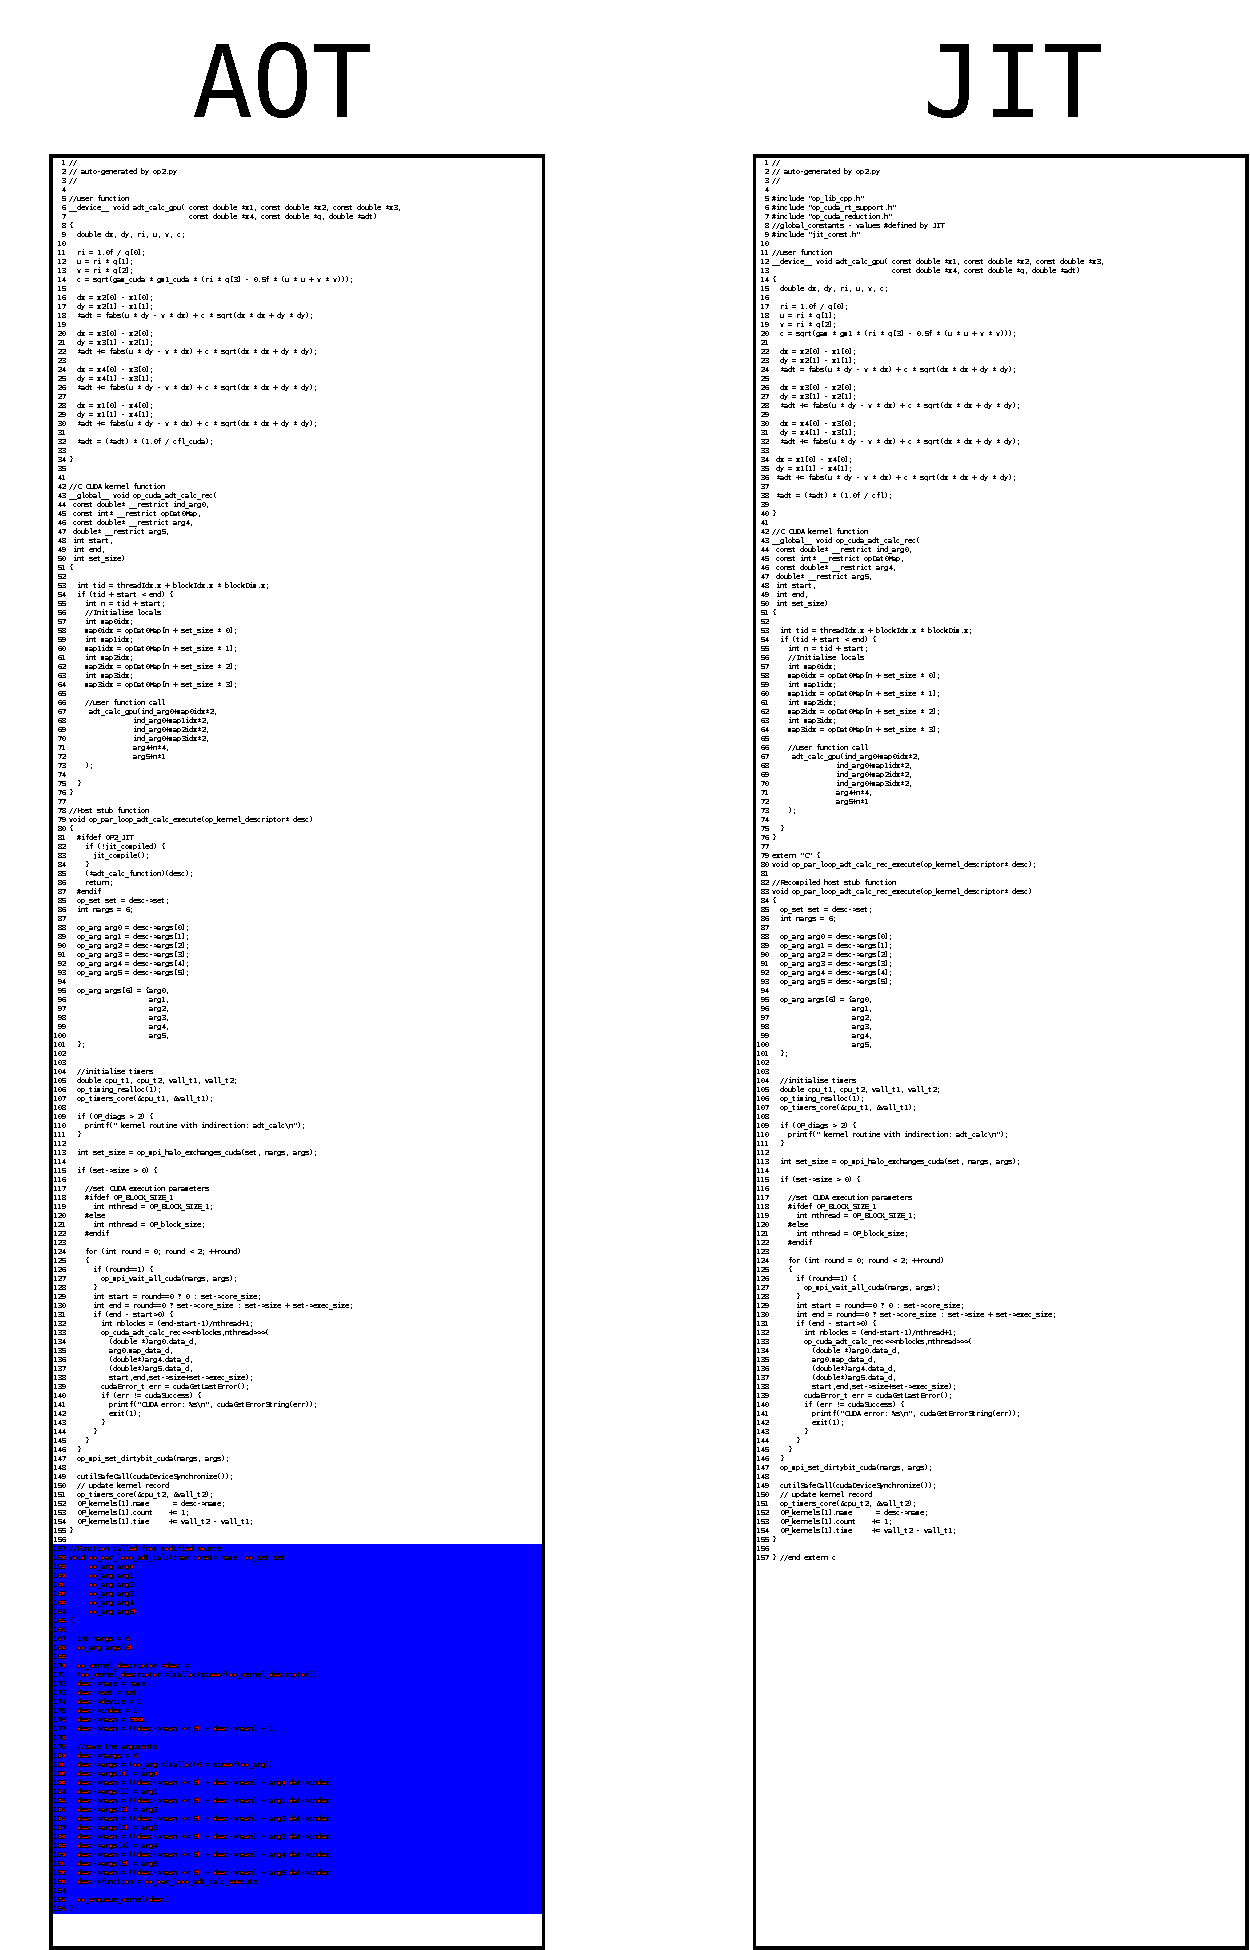
\includegraphics[width=.3\textwidth]{loop_function}
\end{wrapfigure}
\minititle{Loop Function}
The last section to be generated in the kernel files for each parallel loop is the Loop Function, which serves as the entry point for the whole loop operation:
\codeline{op_par_loop_[name](char* name, op_set set, [args]... )}{}

\noindent The application file will be modified by \verb|op2.py| to contain an declaration for this function marked \verb|extern|, to be linked againt this definition. Only the AOT kernel requires this, as previously mentioned the Host Function acts as the entry point for the JIT compiled kernel.
\\
The purpose of this function is to generate the kernel descriptor for the loop. This is an OP2 data structure that contains the name, operating set, arguments, and execution function of the loop, which is passed as an argument to:
\codeline{void op_enqueue_kernel(op_kernel_descriptor *desc)}{op2/c/src/core/op\_lazy.cpp [71-89]}

As previously mentioned, the kernel descriptor and enqueue function were part of the work done to enable lazy execution in OP2, and not created as part of this project.

\clearpage

\subsubsection{Kernel Files Summary}
\label{impl_summary}

To summerise, for every parallel loop two seperate kernel files containing C code are generated, one for Ahead of Time compilation, and one for Just in Time compilation. The code will to be executed when that loop is invoked in the application file, which has been modified to match the function signatures, so the compiler can link the two together.

\begin{wrapfigure}{r}{.42\textwidth}
  \centering
  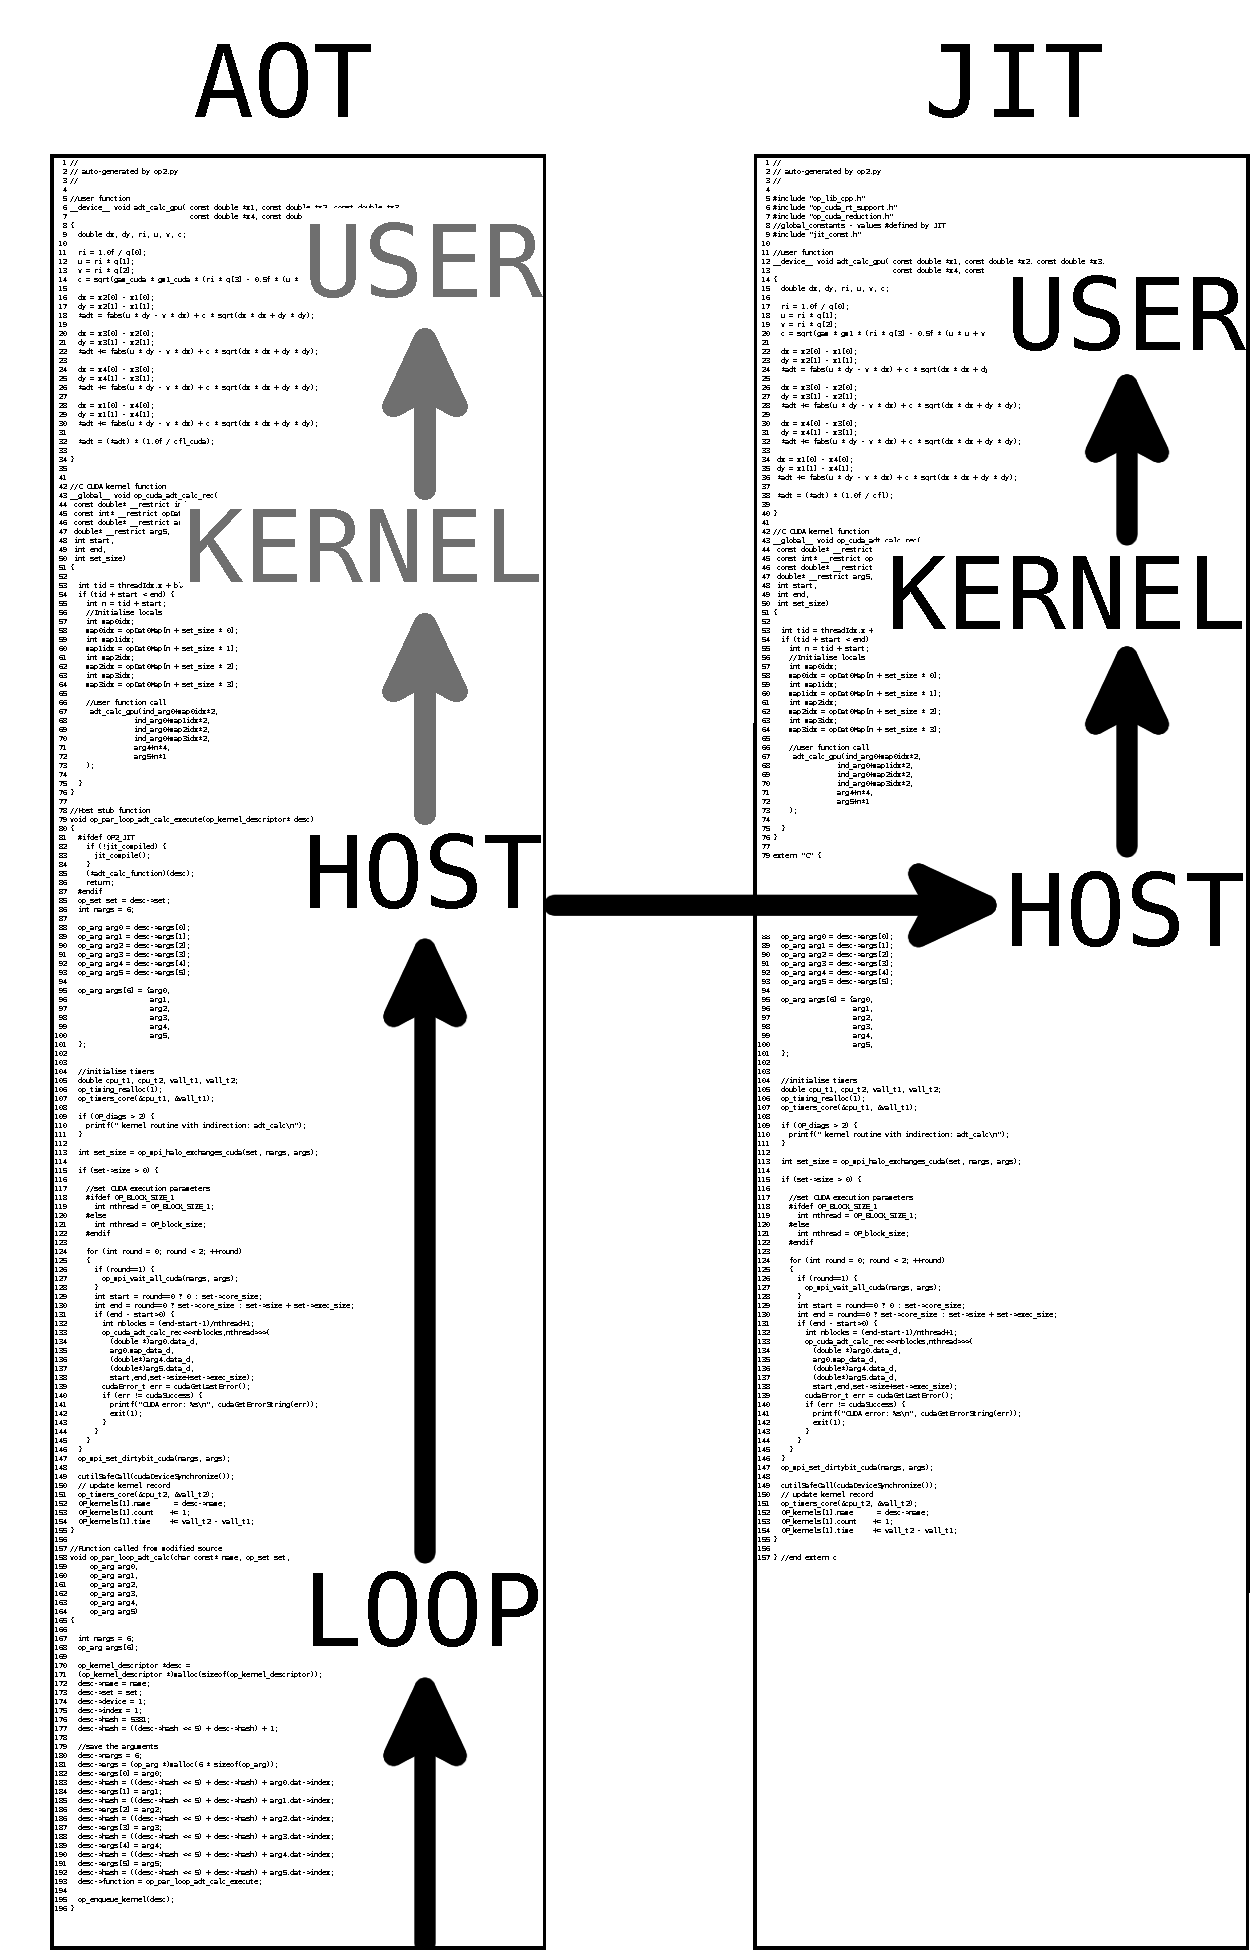
\includegraphics[width=.39\textwidth]{krnl_flow}
  \caption{Kernel Flow}
  \label{fig:krnl_flow}
\end{wrapfigure}

Figure \ref{fig:krnl_flow} has been included to clarify the data flow through the two files: starting in the Loop Function at the bottom, which calls the AOT Host Function, where either the re-compiled JIT version is invoked, or the original version is used if JIT compilation is not enabled at when the application is compiled. In the host function the GPU device is invoked, creating many parallel threads, each executing the Kernel and User functions simultaneously.

The \verb|jit_compile()| function, which is called by the AOT compiled kernel's Host Function when the run-time compilation should happen, has not yet been defined. This will be covered in the next section on the final source file to be generated: the central kernels file.
\clearpage
\subsubsection{Central Kernels File}
\label{sss:mkf}
The Central Kernels File: \verb|cuda/[application]_kernels.cu| is the last file to be generated, once the kernels for each parallel loop have been completed. It ties up most of the remaining loose ends, as it contains shared functions for invoking the run-time compiler, and declaring constants. It also contains \verb|#include| statements for each of the AOT kernel files, so their contents is imported to make a single file.
\par
When this file is included by the application, the linker will be able to find definitions for each of the parallel loop functions, which were declared extern in the Modified Application File. The compilation process for generated code will be covered further in Section \ref{ss:make} on the Makefile.
\par
At the top, the central kernels file includes the requried OP2 library files. It then defines a CUDA constant for each constant the user has defined, which is generated using the following python code:\\
\begin{lstlisting}[backgroundcolor = \color{lightgray!20}, language=Python]
for nc in range (0,len(consts)):
  if consts[nc]['dim']==1:
    # __constant__ [type] [name]_cuda;
    code('__constant__ ' + consts[nc]['type'][1:-1] + ' ' +
          consts[nc]['name'] + '_cuda;')
  else:
    if consts[nc]['dim'] > 0:
      num = str(consts[nc]['dim'])
    else:
      num = 'MAX_CONST_SIZE'

    # __constant__ [type] [name]_cuda[ [dim] ];
    code('__constant__ ' + consts[nc]['type'][1:-1] + ' ' +
          consts[nc]['name'] + '_cuda' + '['+num+'];')
\end{lstlisting}
\codelabel{translator/c/python/jit/op2\_gen\_cuda\_jit.py [974-985]}
\clearpage

\begin{lstlisting}
__constant__ double gam_cuda;
__constant__ double gm1_cuda;
__constant__ double cfl_cuda;
__constant__ double eps_cuda;
__constant__ double mach_cuda;
__constant__ double alpha_cuda;
__constant__ double qinf_cuda[4];
\end{lstlisting}
\vspace{-1cm}
\codelabel{example output of previous code segment}

Following this, the file contains definitions for two functions. The first is the OP2 API function \verb|op_decl_const_char|, which will be called from the application file to declare a constant identifier and value; and the second is \verb|jit_compile| which will invoke the run-time compiler, load the generated shared object file, and assign a function pointer for each re-compiled loop exported by the DLL so it can be found an executed when required.

\minititle{op\_decl\_const\_char}
This function is an OP2 API function which allows users to declare an input value that will not change over the course of execution. It currently has the following signature, as defined in the OP2 User Guide \cite[p9]{manual}:
\codeline{void op_decl_const_char(int dim, char const *type, int size,
                                  char *dat, char const *name)}{}
 Two versions of the function are generated, but only one will be used depeneding on whether JIT compilation is enabled or disabled. The two functions definitions are wrapped with pre-processor conditionals, so that only one of them will be visible to the compiler. As before, the \verb|OP2_JIT| flag being defined is the condition for the JIT functionality to be enabled.


\par
The version of the function for when JIT compilation is disabled is based on the exisiting code generation, and so copies the value passed to it to the corresponding device constant using:
\codeline{cudaMemcpyToSymbol(const void* symbol, const void* src, size_t count)}{}
\noindent The default copy direction for this function is from host memory to device memory, so it does not need to be passed as a parameter.
\par
The JIT version instead invokes the internal library function:
\codeline{void op_lazy_const(int dim, char const *type, int typeSize, char *data,
                        char const *name)}{op2/c/src/core/op\_lazy.cpp [100-101]}
Which maintains a de-duplicated list of constants, so that once they all have been declared the header file defining their values can be generated. As can be seen in the generated C code below, constants containing more than one value are declared as single values due to the issues with \verb|extern __constant__| values described in Section \ref{ss:krnl_files} (2. User Function).
\begin{lstlisting}[linewidth = \textwidth, framesep=0pt]
void op_decl_const_char(int dim, char const *type,
                        int size, char *dat,
                        char const *name)
{
  if (dim == 1) {
    op_lazy_const(dim, type, size, dat, name);
  }
  else {
    for (int d = 0; d < dim; ++d)
    {
      char name2[32];
      sprintf(name2, "op_const_%s_%d\0", name, d);
      op_lazy_const(1, type, size, dat+(d*size), name2);
    }
  }
}
\end{lstlisting}
\vspace{-1em}
\hspace*{\fill}\footnotesize{generated by translator/c/python/jit/op2\_gen\_cuda\_jit.py [1028-1046]}

\minititle{jit\_compile}
The other function generated is the \verb|jit_compile| function, which is responsible for the actual recompilation of the JIT kernels, and making their functions available to the binary. It also uses the same timing library functions which gather data on the time spent in each parallel loop to determine how long the binary spends re-compiling, as this is important for performance measuring later.
\par
The compiler arguments, library paths, and other required parameters are in this implementation handled by a make file which would need to be generated by the user. The contents of the makefile will be covered in the next section.
\par
As can be seen below, the executable makes a system call to initiate a make command, and stores the result in a log file. If the compilation fails, an error message is printed, and the program exits early.
\begin{lstlisting}[linewidth = \textwidth, framesep=0pt]
if (op_is_root()) {
  if (system("make -j [application]_cuda_rec &> jit_compile.log"))
  {
    // 0 indicated success
    printf("Error: JIT compile failed. \n
            - see jit_compile.log for details\n");
    exit(1);
  }
}
\end{lstlisting}
\vspace{-1em}
\hspace*{\fill}\footnotesize{generated by translator/c/python/jit/op2\_gen\_cuda\_jit.py [1071-1077]}

It is expected that the make file will generate a shared object file named \verb|cuda/airfoil_kernel_rec.so|. If this file does not exist the binary exits with an error, otherwise the recompiled function for each parallel loop is dynamically loaded using:
\codeline{void *dlsym(void *restrict handle, const char *restrict name);}{dlfcn.h}
The function \verb|op_par_loop_[name]_rec_execute| loaded, with the address stored in a void pointer with identifer \verb|[name]_function|. We have seen this pointer before in Section \ref{ss:krnl_files} (4. Host Function).
\par
Once this has been done for all loops, the wall clock time since the start of the \verb|jit_compile| function is printed to the terminal.

\subsection{Makefile}
\label{ss:make}
This implementation relies on GNU Make\cite{make} to determine which compiler should be used, which parameters should be passed, and other options. There are a number of libraries required to build an OP2 binary, as covered in Appendix \ref{app:getStart}, so only the recompilation target will be discussed here.
\par
The binary expects there to be a Makefile in the directory it executes in, with a target: \verb|[application]_cuda_rec| in order to work correctly. This is the target which will be compiled at run-time. As mentioned in the previous section, the result of making this target needs to be a a shared object file named \verb|cuda/airfoil_kernel_rec.so|, which contains the recompiled loop functions.
\par
The library object is produced by compiling each of the kernels individually, using the NVidia compiler \verb|nvcc| from the NVidia CUDA Toolkit\cite{nvcc,toolkit} as the code contains CUDA, then linking them into a single object. It is necessary that the compiler flags include \verb|--compiler-options -fPIC|. This passes a list of arguments to the underlying compiler, since nvcc only handles the CUDA code, and passes all host code compilation on to a C compiler. The argument to be passed down is \verb|-fPIC|, to generate Position Independant Code, to allow the library function to execute correctly, regardless of the address at which it is loaded in memory.
\subsubsection{Optional Functionality}
By default, the JIT compilation functionality is enabled in the Makefile by setting the value of \verb|$JIT| to \verb|TRUE|. However, if the variable is set to anything else in the parameters of the make command, JIT will be disabled in the resulting executable. This is done with the following lines:
\begin{lstlisting}[linewidth = \textwidth, framesep=0pt]
ifeq ($(JIT), TRUE)
	CCFLAGS    := $(CCFLAGS) -DOP2_JIT
	NVCCFLAGS  := $(NVCCFLAGS) -DOP2_JIT
	SUFFIX     := _jit
endif
\end{lstlisting}
Which adds a parameter to the C and CUDA compilers to define \verb|OP2_JIT| for the preprocessor, and appends "\_jit" to the name of the executable generated.
\par
The target \verb|cuda/airfoil_kernels_cu.o| is also declared PHONY, so that it is always recompiled even if the file already exists, otherwise this make flag would not function correctly, and a JIT enabled version of this file may be used when the user intended to recompile it with JIT disabled.
